\documentclass[crop=false]{standalone}
%\documentclass{standalone}
\usepackage{tikz} % To generate the plot from csv
\usepackage{pgfplots}
\usepackage{graphicx}
\usepackage{booktabs}
\usepackage{subfig}
\usepackage{float}
\usepackage[section]{placeins} % getting figures below sections
\usepackage{blindtext}
\usepackage{siunitx}
\usepgfplotslibrary{units} % Allows to enter the units nicely
\usetikzlibrary{external} %https://tex.stackexchange.com/questions/1460/script-to-automate-externalizing-tikz-graphics
\tikzexternalize[prefix=savedfigures/]

\pgfplotsset{compat=newest} % Allows to place the legend below plot
\usepackage{pgfplotstable}
\usepgfplotslibrary{statistics}

% #################### Function definition for box plots read table ##################\
\makeatletter
\pgfplotsset{
	boxplot prepared from table/.code={
		\def\tikz@plot@handler{\pgfplotsplothandlerboxplotprepared}%
		\pgfplotsset{
			/pgfplots/boxplot prepared from table/.cd,
			#1,
		}
	},
	/pgfplots/boxplot prepared from table/.cd,
	table/.code={\pgfplotstablecopy{#1}\to\boxplot@datatable},
	row/.initial=0,
	make style readable from table/.style={
		#1/.code={
			\pgfplotstablegetelem{\pgfkeysvalueof{/pgfplots/boxplot prepared from table/row}}{##1}\of\boxplot@datatable
			\pgfplotsset{boxplot/#1/.expand once={\pgfplotsretval}}
		}
	},
	make style readable from table=lower whisker,
	make style readable from table=upper whisker,
	make style readable from table=lower quartile,
	make style readable from table=upper quartile,
	make style readable from table=median,
	make style readable from table=average,
	make style readable from table=lower notch,
	make style readable from table=upper notch
}
\makeatother
\begin{document}

\section{3 2 Mumford0 GA Mutations 20210718 131558}

% ######################## UTRP GA Mutation operators applied ######################## 
\begin{figure} 
\centering 
\tikzsetnextfilename{UTRP_NSGAII_BP_mutation_funcs_phd} 
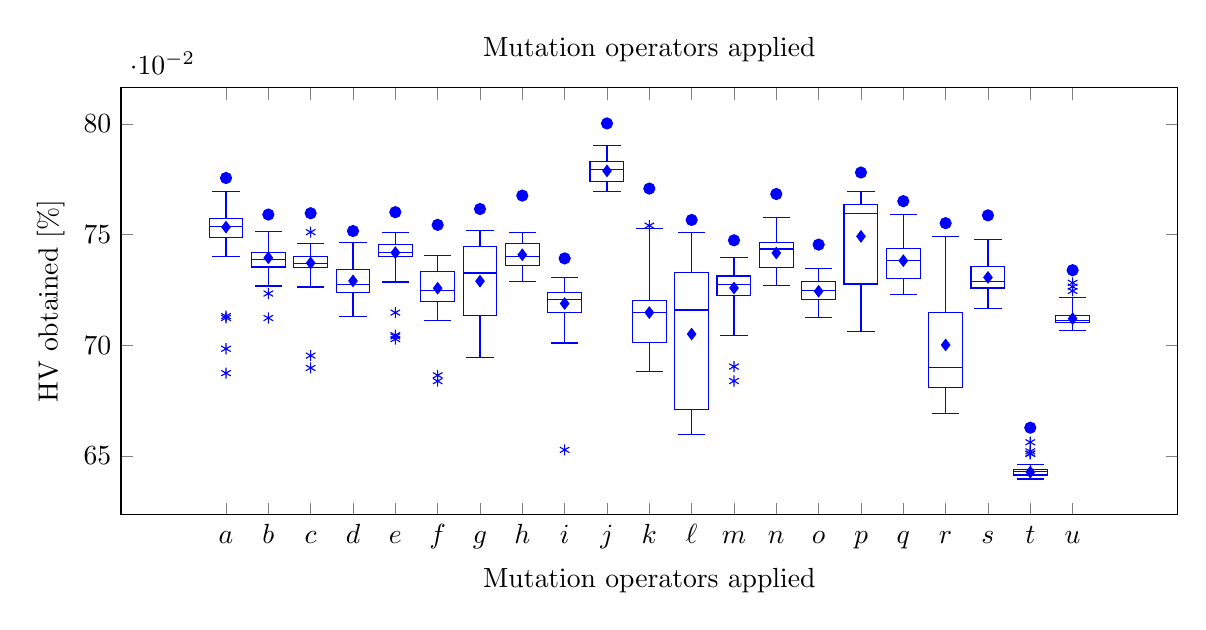
\begin{tikzpicture} 
\begin{axis}[ 
title={Mutation operators applied}, 
boxplot/draw direction=y, 
xtick={1,2,3,4,5,6,7,8,9,10,11,12,13,14,15,16,17,18,19,20,21}, 
%xticklabels={\vphantom{b}{a},\vphantom{b}{b},\vphantom{b}{c},d,\vphantom{b}{e},f,\vphantom{b}{g},h,\vphantom{b}{i},\vphantom{b}{j},k,l,\vphantom{b}{m},\vphantom{b}{n},\vphantom{b}{o},\vphantom{b}{p},\vphantom{b}{q},\vphantom{b}{r},\vphantom{b}{s},\vphantom{b}{t},\vphantom{b}{u}}, 
xticklabels={\vphantom{$b$}{$a$},\vphantom{$b$}{$b$},\vphantom{$b$}{$c$},$d$,\vphantom{$b$}{$e$},$f$,\vphantom{$b$}{$g$},$h$,\vphantom{$b$}{$i$},\vphantom{$b$}{$j$},$k$,$\ell$,\vphantom{$b$}{$m$},\vphantom{$b$}{$n$},\vphantom{$b$}{$o$},\vphantom{$b$}{$p$},\vphantom{$b$}{$q$},\vphantom{$b$}{$r$},\vphantom{$b$}{$s$},\vphantom{$b$}{$t$},\vphantom{$b$}{$u$}}, 
x tick label style={rotate=0, align=center}, 
xlabel={Mutation operators applied}, 
scaled y ticks={base 10:2}, %y tick label style={/pgf/number format/.cd,fixed,precision=3, zerofill}, 
ylabel={HV obtained [\%]}, 
height=7cm,
width=15cm
] 

% ############## Mutations=1 ################## 
\addplot[boxplot, mark=asterisk, 
boxplot prepared={ 
lower whisker=0.74017, 
upper whisker=0.76939, 
lower quartile=0.74851, 
upper quartile=0.75726, 
median=0.75369, 
average=0.75337}, 
color = blue, solid, area legend] 
coordinates {
(2,0.6984)
(2,0.68738)
(2,0.71232)
(2,0.71315)}; 
\addplot[only marks,mark=*,color = blue]coordinates{(1,0.77553)}; 

% ############## Mutations=2 ################## 
\addplot[boxplot, mark=asterisk, 
boxplot prepared={ 
lower whisker=0.72674, 
upper whisker=0.75126, 
lower quartile=0.73531, 
upper quartile=0.74168, 
median=0.73879, 
average=0.73951}, 
color = blue, solid, area legend] 
coordinates {
(3,0.72334)
(3,0.71229)}; 
\addplot[only marks,mark=*,color = blue]coordinates{(2,0.75903)}; 

% ############## Mutations=4 ################## 
\addplot[boxplot, mark=asterisk, 
boxplot prepared={ 
lower whisker=0.7263, 
upper whisker=0.74583, 
lower quartile=0.73524, 
upper quartile=0.74004, 
median=0.73693, 
average=0.73715}, 
color = blue, solid, area legend] 
coordinates {
(5,0.6953)
(5,0.75107)
(5,0.68972)}; 
\addplot[only marks,mark=*,color = blue]coordinates{(3,0.75962)}; 

% ############## Mutations=5 ################## 
\addplot[boxplot, mark=asterisk, 
boxplot prepared={ 
lower whisker=0.71302, 
upper whisker=0.74657, 
lower quartile=0.72365, 
upper quartile=0.73433, 
median=0.7275, 
average=0.72905}, 
color = blue, solid, area legend] 
coordinates {}; 
\addplot[only marks,mark=*,color = blue]coordinates{(4,0.75158)}; 

% ############## Mutations=3 ################## 
\addplot[boxplot, mark=asterisk, 
boxplot prepared={ 
	lower whisker=0.72857, 
	upper whisker=0.75087, 
	lower quartile=0.74002, 
	upper quartile=0.74538, 
	median=0.7419, 
	average=0.74182}, 
color = blue, solid, area legend] 
coordinates {
	(4,0.71472)
	(4,0.70277)
	(4,0.70394)
	(4,0.70454)}; 
\addplot[only marks,mark=*,color = blue]coordinates{(5,0.7601)}; 

% ############## Mutations=6 ################## 
\addplot[boxplot, mark=asterisk, 
boxplot prepared={ 
lower whisker=0.71114, 
upper whisker=0.7405, 
lower quartile=0.71968, 
upper quartile=0.73317, 
median=0.72481, 
average=0.72576}, 
color = blue, solid, area legend] 
coordinates {
(7,0.68376)
(7,0.68639)}; 
\addplot[only marks,mark=*,color = blue]coordinates{(6,0.75436)}; 

% ############## Mutations=7 ################## 
\addplot[boxplot, mark=asterisk, 
boxplot prepared={ 
lower whisker=0.69456, 
upper whisker=0.75199, 
lower quartile=0.71346, 
upper quartile=0.7446, 
median=0.7326, 
average=0.72892}, 
color = blue, solid, area legend] 
coordinates {}; 
\addplot[only marks,mark=*,color = blue]coordinates{(7,0.76152)}; 

% ############## Mutations=8 ################## 
\addplot[boxplot, mark=asterisk, 
boxplot prepared={ 
lower whisker=0.72858, 
upper whisker=0.75107, 
lower quartile=0.73589, 
upper quartile=0.7461, 
median=0.74022, 
average=0.74086}, 
color = blue, solid, area legend] 
coordinates {}; 
\addplot[only marks,mark=*,color = blue]coordinates{(8,0.76759)}; 

% ############## Mutations=9 ################## 
\addplot[boxplot, mark=asterisk, 
boxplot prepared={ 
lower whisker=0.70098, 
upper whisker=0.7307, 
lower quartile=0.71475, 
upper quartile=0.72371, 
median=0.7205, 
average=0.71882}, 
color = blue, solid, area legend] 
coordinates {
(10,0.65271)}; 
\addplot[only marks,mark=*,color = blue]coordinates{(9,0.73921)}; 

% ############## Mutations=0 ################## 
\addplot[boxplot, mark=asterisk, 
boxplot prepared={ 
	lower whisker=0.76952, 
	upper whisker=0.79029, 
	lower quartile=0.77415, 
	upper quartile=0.783, 
	median=0.77951, 
	average=0.77874}, 
color = blue, solid, area legend] 
coordinates {}; 
\addplot[only marks,mark=*,color = blue]coordinates{(10,0.80019)}; 

% ############## Mutations=10 ################## 
\addplot[boxplot, mark=asterisk, 
boxplot prepared={ 
lower whisker=0.68792, 
upper whisker=0.75276, 
lower quartile=0.70142, 
upper quartile=0.72014, 
median=0.71489, 
average=0.71474}, 
color = blue, solid, area legend] 
coordinates {
(11,0.75404)}; 
\addplot[only marks,mark=*,color = blue]coordinates{(11,0.77076)}; 

% ############## Mutations=11 ################## 
\addplot[boxplot, mark=asterisk, 
boxplot prepared={ 
lower whisker=0.65973, 
upper whisker=0.75075, 
lower quartile=0.67083, 
upper quartile=0.73278, 
median=0.71589, 
average=0.70503}, 
color = blue, solid, area legend] 
coordinates {}; 
\addplot[only marks,mark=*,color = blue]coordinates{(12,0.75658)}; 

% ############## Mutations=14 ################## 
\addplot[boxplot, mark=asterisk, 
boxplot prepared={ 
lower whisker=0.7042, 
upper whisker=0.73978, 
lower quartile=0.7223, 
upper quartile=0.73128, 
median=0.72746, 
average=0.72584}, 
color = blue, solid, area legend] 
coordinates {
(15,0.69036)
(15,0.68382)}; 
\addplot[only marks,mark=*,color = blue]coordinates{(13,0.7474)}; 

% ############## Mutations=12 ################## 
\addplot[boxplot, mark=asterisk, 
boxplot prepared={ 
	lower whisker=0.72683, 
	upper whisker=0.75765, 
	lower quartile=0.73495, 
	upper quartile=0.74628, 
	median=0.74344, 
	average=0.74166}, 
color = blue, solid, area legend] 
coordinates {}; 
\addplot[only marks,mark=*,color = blue]coordinates{(14,0.7683)}; 

% ############## Mutations=13 ################## 
\addplot[boxplot, mark=asterisk, 
boxplot prepared={ 
	lower whisker=0.71235, 
	upper whisker=0.73456, 
	lower quartile=0.72052, 
	upper quartile=0.72874, 
	median=0.72471, 
	average=0.72438}, 
color = blue, solid, area legend] 
coordinates {}; 
\addplot[only marks,mark=*,color = blue]coordinates{(15,0.74544)}; 

% ############## Mutations=18 ################## 
\addplot[boxplot, mark=asterisk, 
boxplot prepared={ 
	lower whisker=0.70611, 
	upper whisker=0.7696, 
	lower quartile=0.72767, 
	upper quartile=0.76339, 
	median=0.75947, 
	average=0.74917}, 
color = blue, solid, area legend] 
coordinates {}; 
\addplot[only marks,mark=*,color = blue]coordinates{(16,0.77801)}; 

% ############## Mutations=15 ################## 
\addplot[boxplot, mark=asterisk, 
boxplot prepared={ 
lower whisker=0.72278, 
upper whisker=0.75918, 
lower quartile=0.73011, 
upper quartile=0.74374, 
median=0.73814, 
average=0.7382}, 
color = blue, solid, area legend] 
coordinates {}; 
\addplot[only marks,mark=*,color = blue]coordinates{(17,0.76507)}; 

% ############## Mutations=19 ################## 
\addplot[boxplot, mark=asterisk, 
boxplot prepared={ 
lower whisker=0.66895, 
upper whisker=0.74899, 
lower quartile=0.68103, 
upper quartile=0.71479, 
median=0.68978, 
average=0.70011}, 
color = blue, solid, area legend] 
coordinates {}; 
\addplot[only marks,mark=*,color = blue]coordinates{(18,0.75514)}; 

% ############## Mutations=16 ################## 
\addplot[boxplot, mark=asterisk, 
boxplot prepared={ 
	lower whisker=0.71647, 
	upper whisker=0.74763, 
	lower quartile=0.72585, 
	upper quartile=0.73541, 
	median=0.72882, 
	average=0.73063}, 
color = blue, solid, area legend] 
coordinates {}; 
\addplot[only marks,mark=*,color = blue]coordinates{(19,0.75866)}; 

% ############## Mutations=20 ################## 
\addplot[boxplot, mark=asterisk, 
boxplot prepared={ 
lower whisker=0.63957, 
upper whisker=0.64628, 
lower quartile=0.64134, 
upper quartile=0.64372, 
median=0.64278, 
average=0.64267}, 
color = blue, solid, area legend] 
coordinates {
(21,0.65105)
(21,0.65203)
(21,0.65091)
(21,0.65615)}; 
\addplot[only marks,mark=*,color = blue]coordinates{(20,0.66273)}; 

% ############## Mutations=17 ################## 
\addplot[boxplot, mark=asterisk, 
boxplot prepared={ 
	lower whisker=0.70665, 
	upper whisker=0.72137, 
	lower quartile=0.71022, 
	upper quartile=0.71357, 
	median=0.71114, 
	average=0.712}, 
color = blue, solid, area legend] 
coordinates {
	(18,0.72451)
	(18,0.72818)
	(18,0.72645)}; 
\addplot[only marks,mark=*,color = blue]coordinates{(21,0.73389)}; 

\end{axis}
\end{tikzpicture}
\end{figure} 
\begin{table}
\centering
\caption{Legend for the boxplot.}
\begin{tabular}{ll}
\toprule
 Index &                      Name \\
\midrule
     0 &          [Intertwine\_two] \\
     1 &              [Add\_vertex] \\
     2 &           [Delete\_vertex] \\
     3 &    [Invert\_path\_vertices] \\
     4 &    [Insert\_inside\_vertex] \\
     5 &    [Delete\_inside\_vertex] \\
     6 &  [Relocate\_inside\_vertex] \\
     7 &   [Replace\_inside\_vertex] \\
     8 &   [Donate\_between\_routes] \\
     9 &     [Swap\_between\_routes] \\
    10 &         [Merge\_terminals] \\
    11 &      [Repl\_low\_dem\_route] \\
    12 &    [Rem\_low\_dem\_terminal] \\
    13 &   [Rem\_lrg\_cost\_terminal] \\
    14 &            [Repl\_subsets] \\
    15 &    [Trim\_one\_terminal\_cb] \\
    16 & [Trim\_one\_path\_random\_cb] \\
    17 &   [Trim\_routes\_random\_cb] \\
    18 &    [Grow\_one\_terminal\_cb] \\
    19 & [Grow\_one\_path\_random\_cb] \\
    20 &   [Grow\_routes\_random\_cb] \\
\bottomrule
\end{tabular}
\end{table}

\begin{table}
	\centering
	\caption{Legend for the boxplot.}
	\begin{tabular}{ll}
		\toprule
		Index &                      Name \\
		\midrule
		1 &              [Add\_vertex] \\
		2 &           [Delete\_vertex] \\
		4 &    [Insert\_inside\_vertex] \\
		5 &    [Delete\_inside\_vertex] \\
		3 &    [Invert\_path\_vertices] \\
		6 &  [Relocate\_inside\_vertex] \\
		7 &   [Replace\_inside\_vertex] \\
		8 &   [Donate\_between\_routes] \\
		9 &     [Swap\_between\_routes] \\
		0 &          [Intertwine\_two] \\
		10 &         [Merge\_terminals] \\
		11 &      [Repl\_low\_dem\_route] \\
		14 &            [Repl\_subsets] \\
		12 &    [Rem\_low\_dem\_terminal] \\
		13 &   [Rem\_lrg\_cost\_terminal] \\
		18 &    [Grow\_one\_terminal\_cb] \\
		15 &    [Trim\_one\_terminal\_cb] \\
		19 & [Grow\_one\_path\_random\_cb] \\
		16 & [Trim\_one\_path\_random\_cb] \\
		20 &   [Grow\_routes\_random\_cb] \\
		17 &   [Trim\_routes\_random\_cb] \\
		\bottomrule
	\end{tabular}
\end{table}

\begin{table}
	\centering
	\caption{Coordinate conversion.}
	\begin{tabular}{rll}
		\toprule
		From & To & Adjustment\\
		\midrule
		1  & 0  & $+1$\\
		2  & 1  & $+1$\\
		4  & 2  & $+1$\\
		5  & 3  & $+1$\\
		3  & 4  & $+1$\\
		6  & 5  & $+1$\\
		7  & 6  & $+1$\\
		8  & 7  & $+1$\\
		9  & 8  & $+1$\\
		0  & 9  & $+1$\\
		10 & 10 & $+1$\\
		11 & 11 & $+1$\\
		14 & 12 & $+1$\\
		12 & 13 & $+1$\\
		13 & 14 & $+1$\\
		18 & 15 & $+1$\\
		15 & 16 & $+1$\\
		19 & 17 & $+1$\\
		16 & 18 & $+1$\\
		20 & 19 & $+1$\\
		17 & 20 & $+1$\\
		\bottomrule
	\end{tabular}
\end{table}

\end{document}
